% Section IV - Methods. SOURCE OF TRUTH (the .md draft is superseded).
% Budget: ~760 total (option B) or ~620 (option A); see word_budget_MLESP.md, advisor Q2.
% Numbers come from 03_Phase3_Corpus/prisma_counts.json and 05_Phase5_Analysis/analysis.py - never type them by hand.

\subsection{Search and screening}
% REVIEW 2026-11-07 (8-page limit): condensed into one paragraph. No criterion or count dropped.
The starting corpus was a previously assembled set of the 100 most-cited articles returned by a Web of Science search on EEG, connectivity, deep learning and depression. Records were screened on title and abstract, then full text, against six criteria, all of which had to hold: (1) EEG is the primary modality; (2) a functional or effective connectivity measure is computed---coherence, PLV, PLI, correlation, Granger causality, mutual information, or a graph derived from one; (3) a deep learning model is applied to those features; (4) the study classifies depression or predicts its severity; (5) at least one quantitative performance metric is reported; and (6) the work is peer-reviewed, in English, and published in 2015 or later. Criterion 2 required at least one edge weight to depend on the recorded signals, so a graph fixed by electrode positions or an atlas did not qualify however the paper described it. Because fewer than 15 Web of Science studies had qualified, the protocol's supplementary search was run in OpenAlex and PubMed in September 2026; retrieval then stopped once the corpus reached 15, a stopping rule the protocol did not specify, so \NwosNotRetrieved{} screened-in Web of Science reports were never assessed at full text, one because no copy was available to us. Fig.~\ref{fig:prisma} gives the counts and exclusion reasons.

\begin{figure}[t]
\centering
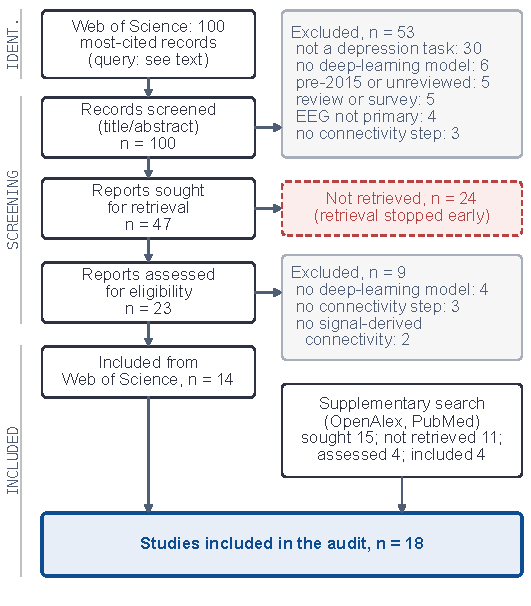
\includegraphics[width=0.80\columnwidth]{figures/fig1_prisma.pdf}
% REVIEW 2026-09-27 (C10): 0.86 width; check legibility
\caption{PRISMA-style screening flow: records at each stage and the reasons for exclusion, generated from the screening log. It is not a systematic review's flow---the starting set was citation-ranked and retrieval incomplete (Section~\ref{sec:discussion}). The supplementary search was run when fewer than 15 studies had qualified, and retrieval stopped at 15 (Section~\ref{sec:methods}). Each of the 100 records is counted once. The dashed box marks reports not retrieved.}
\label{fig:prisma}
\end{figure}

\subsection{Extraction fields}
% REVIEW 2026-11-07 (8-page limit): the three paragraphs below were condensed into two. No field dropped.
The coding sheet's columns were fixed before any study was coded. Descriptive fields recorded the citation; the dataset (MODMA, PRED+CT, the Mumtaz resting-state dataset, a private cohort, or other); total, MDD and control sample sizes; the connectivity measure; the frequency bands; and the architecture family. Pipeline fields recorded whether recordings were epoched and how many epochs each subject contributed; the partitioning unit (subject, epoch, or unclear); and the validation strategy (holdout, $k$-fold, leave-one-subject-out, external, or unclear). Four further fields recorded, for each of L2--L5, whether the step was stated to be fit within the training fold, fit on the whole dataset, not performed, or unclear.

Performance fields recorded reported accuracy and other metrics. Where a study reported more than one accuracy, we took the result for the model the paper proposes under the most subject-independent protocol it reports, coded its leakage fields for that same protocol, and preferred the results tables where these disagreed with the abstract. This rule was fixed after the initial coding pass, which had followed each abstract's headline figure, but before any accuracy was analyzed; one study was left on the protocol both raters coded, with the matching accuracy, so that rating and accuracy always refer to the same protocol. The abstract's headline figure was kept as a second field for a sensitivity analysis. Only binary depression-versus-control accuracies enter the primary comparison; other tasks enter a sensitivity analysis.

% REVIEW 2026-09-27 (E3): rule from the rater guide.
% FIX 2026-09-27 (F1): the last sentence was hidden behind the inline comment above; restored.
% FIX 2026-09-27 (F2): the rater sheets hold one evidence_quote per study, not one per field.
For every study each rater recorded an evidence quote, the passage on which the coding rests. Coding drew only on the published text: authors were not contacted and code repositories were not consulted.

% REVIEW 2026-11-07 (R1 points 1 and 3; R2 W6, Q4): the convention and its direction of bias made explicit,
% with a forward pointer to the bound in Section V-D. The coded fields are unchanged.
One convention needs stating plainly, because it is the weakest point of the scheme. A threshold, rescaling or selection step never mentioned was coded not performed; a step mentioned without saying which data it was fit on was coded unclear. Silence does not establish that a step was not performed, so the convention can only move studies toward the leakage-free end, and our sheets record one value for both readings. We therefore do not rely on it: Section~\ref{sec:results} reports the strictest alternative, treating every such silence as unclear, and states which conclusions survive it.

\subsection{Rating scheme}
Each study received one of four ratings, applied from reported methods alone:
\begin{itemize}
\item \emph{Leakage-free}: subject-level partitioning is stated, and connectivity estimation, thresholding, normalization and channel or band selection are each stated to be confined to the training fold or not performed.
\item \emph{Leakage-possible}: subject-level partitioning is stated, but at least one of L2--L5 is not clearly described as within-fold.
\item \emph{Leakage-likely}: partitioning is at epoch level, or a preprocessing step is explicitly applied to the full dataset before partitioning.
\item \emph{Unclear}: the partitioning unit is not stated.
\end{itemize}
Unclear is a category in its own right rather than missing data, because its prevalence is itself a result for RQ1.

Raters did not assign the rating directly: they coded the partitioning unit and the four surface fields, and a fixed rule implemented in code derived the rating, so both raters' ratings follow the same logic. Where rules overlap, leakage-likely takes precedence: an explicit whole-dataset step makes a study leakage-likely whatever its partitioning unit.

Two conventions were fixed before coding and given to both raters in identical written instructions: a threshold applied to each matrix using only that matrix's own values, and normalization computed within each segment, were coded within-fold, since neither draws on other samples; and batch-normalization layers inside a network were not treated as preprocessing.

\subsection{Rater procedure and analysis plan}
Two raters coded every included study independently, without discussion, from identical written instructions. Percentage agreement and unweighted Cohen's $\kappa$ on the four-level rating were computed before any disagreement was discussed. Disagreements were then resolved with a senior researcher as tiebreaker, and both pre- and post-resolution ratings are reported. A $\kappa$ below 0.4 was pre-specified as indicating that the scheme is too subjective to use as defined.

The analysis was specified, and its code written, before accuracies were examined. RQ1, RQ2 and RQ4 are descriptive and no confirmatory test is performed for them. For RQ1 we report the proportion of studies in each reporting category, overall and per surface, with Wilson 95\% confidence intervals. The 95\% interval for $\kappa$ comes from 10{,}000 bootstrap resamples of studies.

% REVIEW 2026-11-07: the four reviewer-requested analyses are declared here as post hoc, so no reader can
% mistake them for part of the pre-specified plan. Code: 05_Phase5_Analysis/reviewer_response.py.
Four analyses were added after review, once ratings and accuracies were known: the strict re-reading above, per-surface agreement, a bootstrap resampling datasets rather than studies, and an exact test for the year trend. They are post hoc, labeled as such wherever they appear, and changed no coded field, rating or pre-specified result.

RQ3 is the only confirmatory analysis. We report median accuracy and interquartile range per rating stratum and compare the leakage-likely and leakage-free strata with a two-sided Mann--Whitney $U$ test, and all strata with a Kruskal--Wallis test, each accompanied by Cliff's $\delta$ with a 10{,}000-resample bootstrap interval. The smallest effect of interest was fixed in advance at 3 percentage points of median accuracy; a smaller difference is reported as a null, and no subgroup was searched for an effect. Because small datasets may both favor weaker partitioning and yield higher accuracy, accuracy by rating is also reported by sample-size tercile. All resampling used a fixed seed, so every reported value can be regenerated from the coding sheet.
